\documentclass[a4paper, 11pt]{article}

% declare packages
\usepackage{amsfonts}
\usepackage{amsmath}
\usepackage{bm}
\usepackage{amssymb}
\usepackage{array}   % write arrays in math mode
\usepackage[margin=10pt,font=small,labelfont=bf]{caption}
% \usepackage[onehalfspacing]{setspace} %[nosep] [noitemsep] [singlespacing] [doublespacing] (also can do /singlespacing within doc)
\usepackage{color}
\usepackage{comment} % enables the use of multi-line comments (\ifx \fi)  
\usepackage{enumitem}
\usepackage{fancyhdr}
\usepackage{footmisc} %  formatting for footnotes
\usepackage{fullpage} %  changes the margin
\usepackage{geometry} %  change length & layout of elements
\usepackage{graphicx} % embed graphics
\usepackage{hyperref}
\usepackage{mathtools} 
\usepackage{multirow}
\usepackage[round,sort,comma]{natbib}   % citation formatting
\usepackage{pdflscape} % make pages landscape in pdf
\usepackage{pdfpages}
% \usepackage{subcaption}
\usepackage{subfigure}
\usepackage{subfloat}   %figure 1a 1b with \begin{subfigures}
\usepackage{ulem} %underlining and strikethroughs
\usepackage[yyyymmdd,hhmmss]{datetime}

% declare extra commands
\DeclarePairedDelimiter\abs{\lvert}{\rvert}%
\DeclarePairedDelimiter\norm{\lVert}{\rVert}%
\DeclareMathOperator*{\argmin}{\arg\!\min}
\DeclareMathOperator*{\argmax}{\arg\!\max}

% Other formatting options
\pagestyle{fancy}
\fancyhf{}
\renewcommand{\headrulewidth}{0pt}
\rfoot{Compiled on \today\ at \currenttime}
\cfoot{}
\lfoot{Page \thepage}
\newcolumntype{L}[1]{>{\raggedright\let\newline\arraybackslash\hspace{0pt}}m{#1}} %used for array package
\newcolumntype{C}[1]{>{\centering\let\newline\arraybackslash\hspace{0pt}}m{#1}}
\newcolumntype{R}[1]{>{\raggedleft\let\newline\arraybackslash\hspace{0pt}}m{#1}}
\geometry{left=1.0in,right=1.0in,top=1.0in,bottom=1.0in}

\begin{document}
% puts extra whitespace at top of first page
% \begin{tabbing}
% \end{tabbing}

\normalsize  \strut\hfill \textbf{John Stromme} \\
\normalsize  \strut\hfill  Date: 07/21 \\

\noindent
\huge \textbf{Do the Bucks actually `play random'?} \\
\textit{An empirical analysis} \\

\normalsize

During halftime in games 1 and 2 of the Finals coach Bud implored his players to `play random'\footnote{\url{https://www.reddit.com/r/nba/comments/ogm608/highlight_mike_budenholzers_game_2_nba_finals/}}. Many internet commentators found this advice to be quite strange and atypical---`play random' is not usually in the wheelhouse of advice that coaches give in rousing halftime speeches. This naturally leads us to two questions: Are the Bud-coached Bucks indeed more likely to `play random' than the other 29 teams in the league? Do teams who `play random' tend to win more games?

To answer these questions, I created a measure of `randomness' of play along two-dimensions using data from the 2019--20 and 2020--21 seasons. On one dimension, teams can be `random' in how far they are from the basket when they have a shot-attempt. A team with more varied shot selection by distance will be much more `random' and unpredictable. On the second dimension, teams can be `random' on \textit{when} they choose to shoot during a possession. Again, a team that is more varied in when they take there shots during a possession will be more `random' and unpredictable than a team who always shoots at a similar point in the shot clock.

Figure \ref{fig:randomgini} shows where each team falls along both dimensions of `randomness': Teams towards the top-right play more `randomly', whereas teams towards the bottom-left play more `predictably'. The bucks play more randomly on both measures than an the nba average. They rank more highly in playing randomly in shot distance, but are closer to the average in shot timing.

\begin{figure}[!htpb]
  \centering 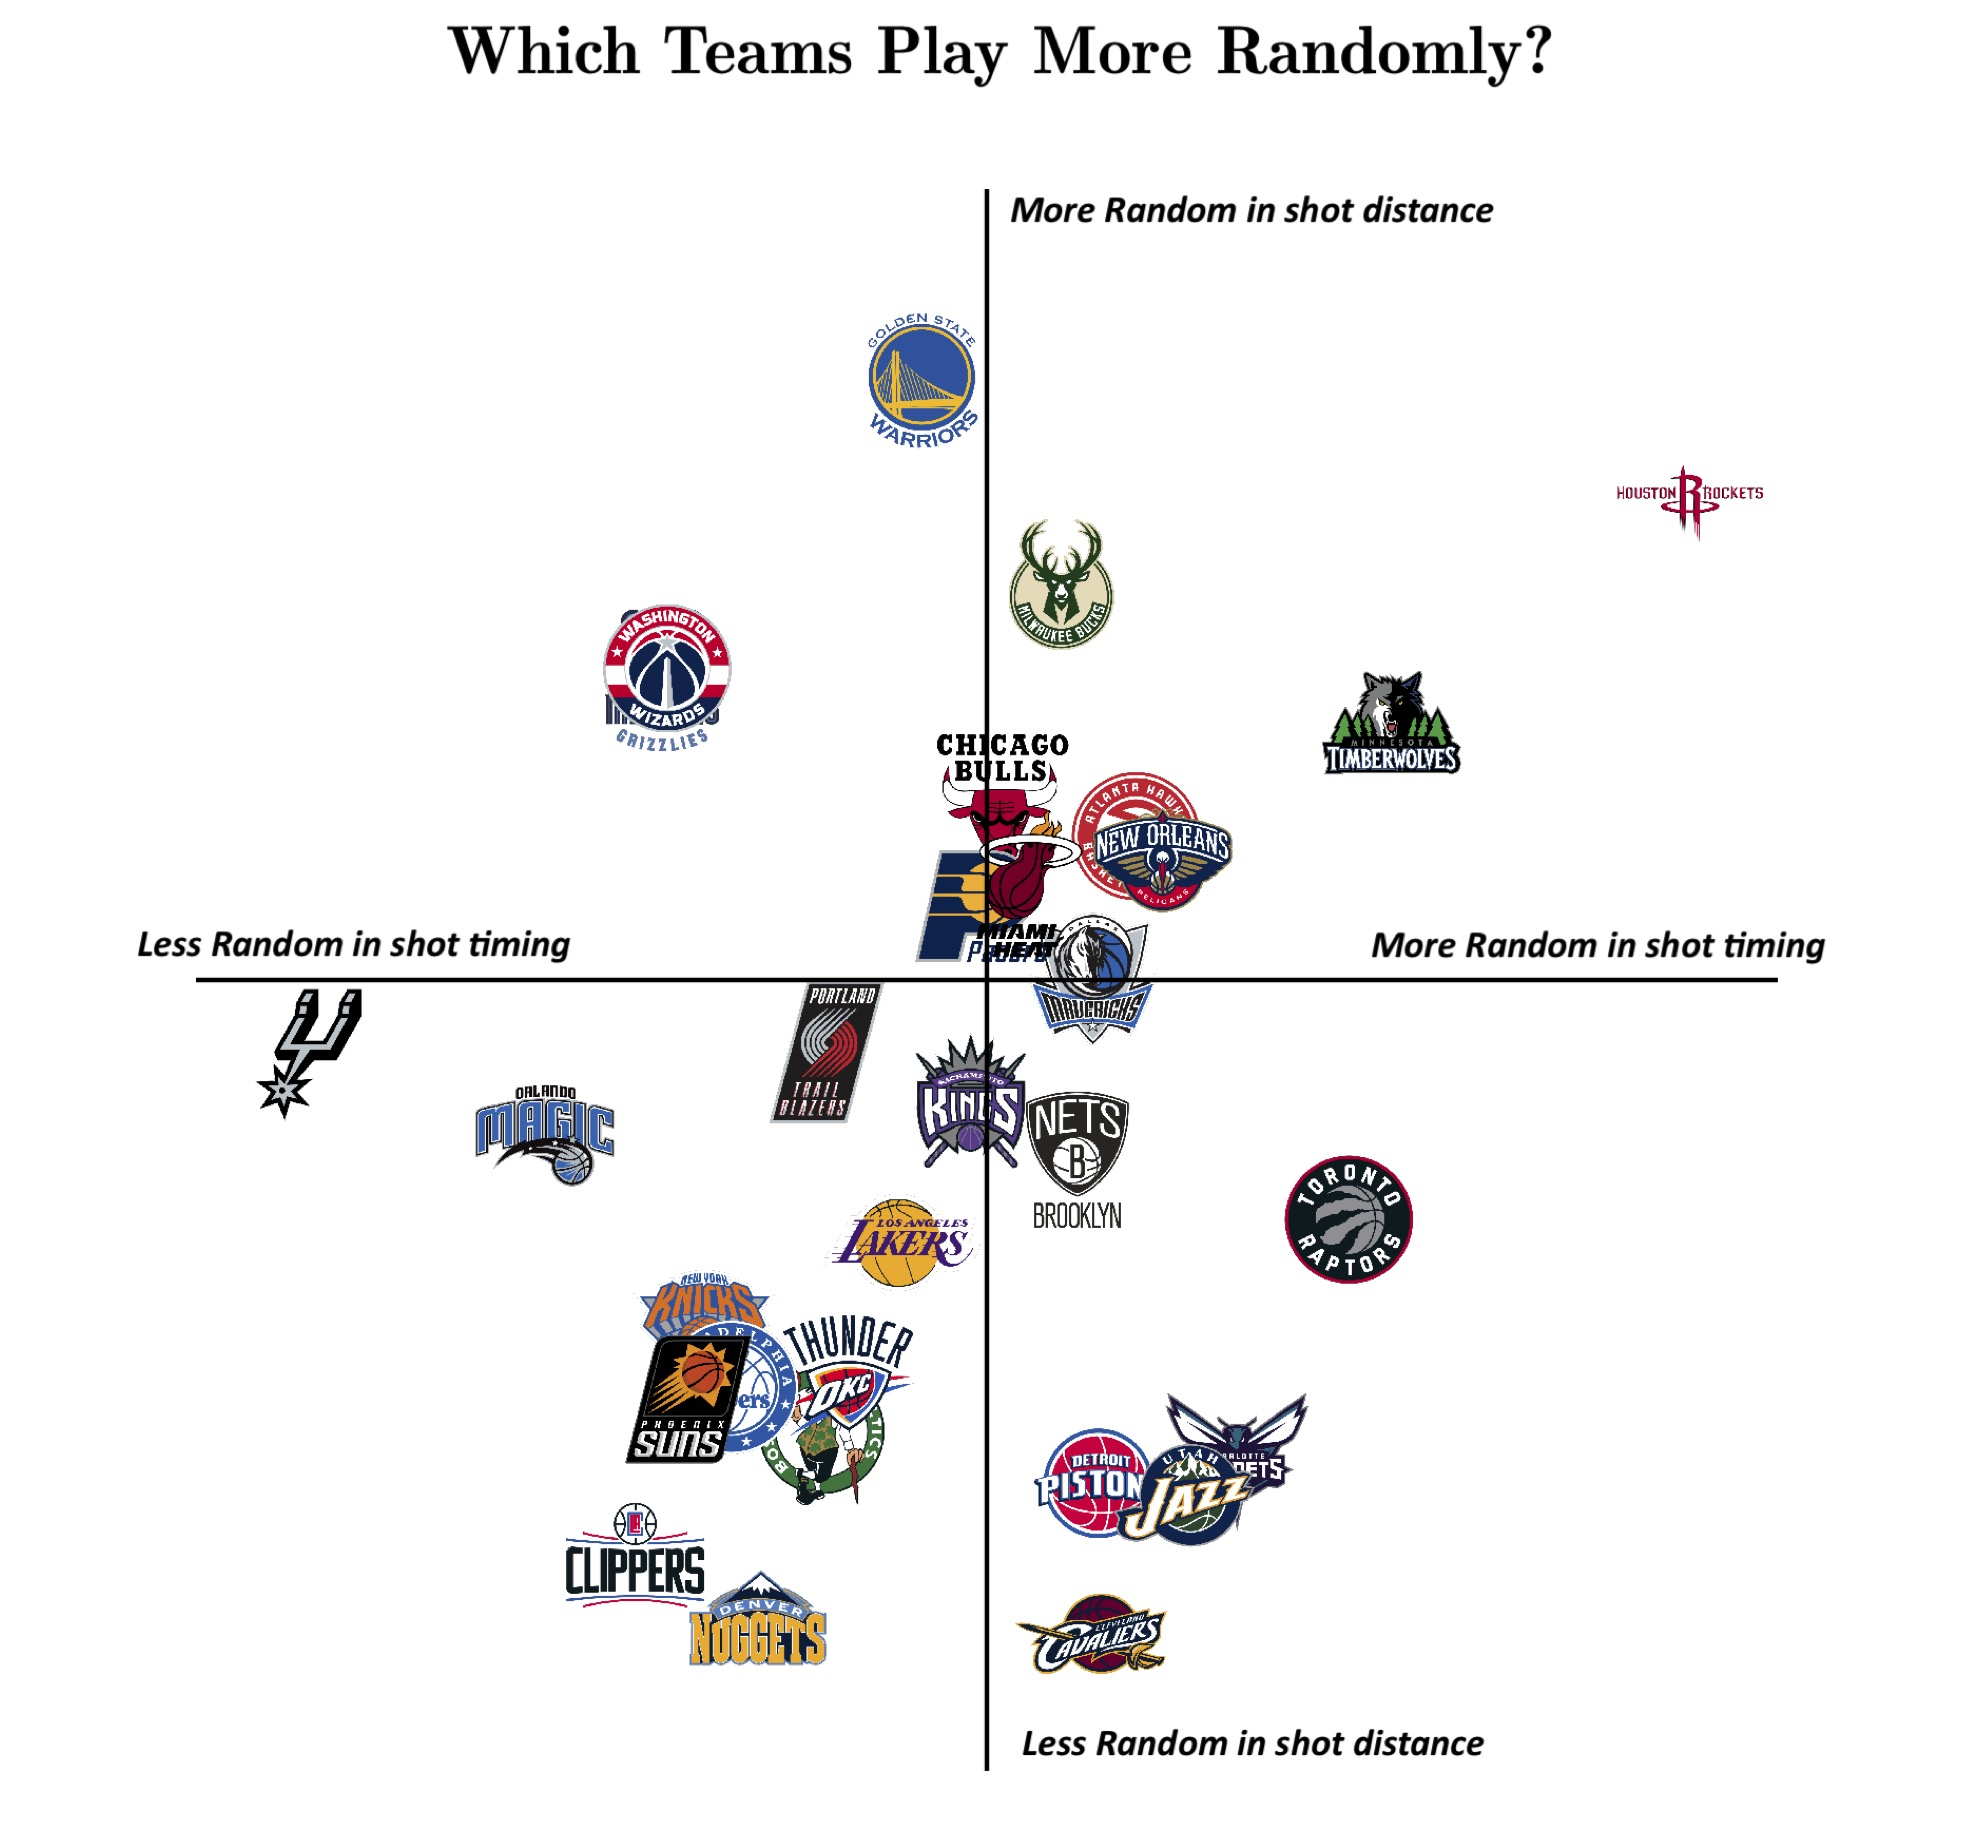
\includegraphics[width=0.6\textwidth]{../plots_tables/randomginiplot.jpg}
  \caption{}\label{fig:randomgini}
\end{figure}




\section*{Is `playing random' correlated with winning?}
It may or may not be a good idea to play `randomly' given that each game a team should exploit opportunities based on matchup. It seems likely there is a tradeoff between exploiting opponent's weaknesses and playing random---more strategic play would be less random. To investigate this I look at the correlation between wins and the above measures of randomness. I find that correlation for each measure is negative: -0.182 for shot distance and -0.235 for shot timing. This implies playing random is associated with losing more games, albeit this correlation is somewhat weak, and no causality is implied.

\section*{Methodology}
For each dimension of randomness, we can think of there being $n$ possible outcomes. For example, a team can choose to shoot at any of the 24 seconds in the shot clock ($n=24$), or at any distance from the basket i.e., between 0--40 feet ($n=40$). If a team is perfectly predictable, they will shoot every shot at the same distance, at the same time in the shot clock. On the opposite end, teams that are most `random' will have an even distribution of shots across distance and time.

A natural measure for this definition of `randomness' is the Gini Coefficient. The Gini coefficient is traditionally used as a measure of income inequality across a population, but can be repurposed anywhere we care about how evenly distributed some piece of data is among some categories or options.

In this application, I'll use what I call the `inverse-Gini Coefficient': the higher the inverse-Gini, the more `random' the team's play is. When the inverse-Gini Coefficient is equal to one, there is an even distribution across possibilities, which, as described in the previous paragraph, is most `random'. At the other extreme, if a team were to only shoot at one distance from the basket (least `random') the inverse-Gini Coefficient would be zero. For the math nerds the formula is further below. %For this analysis, the inverse-Gini Coefficient is multiplied by 100 for easier reading.

\subsection*{The Nitty Gritty}
\noindent\textbf{A note on notation:} For each measure we can use $n$ to represent the number of `options' a team has, and $x_i$ to represent the number of times a team chose option $i$.\\

\noindent \textbf{Shot distance randomness:} Teams can choose to shoot from one of $n=28$ discrete shot distances, either shooting between 0--26 feet, or from `deep' which is a single category for any shot between 27--40 feet. Any shot over 40 feet is dropped from the data. Using the notation defined above, this means that $x_0$ would measure the number of times over a season a team shot from 0-feet.\\

\noindent\textbf{Shot timing randomness:} Teams can choose to shoot from one of $n=20$ times during the shot clock, i.e., at any point between 19--0 seconds left on the shot clock. The first 5 seconds of the shot clock, 24--20, are dropped as a standard length of time to get the ball over halfcourt. Again using the above notation, in this case $x_0$ would measure the number of times over a season a team made a shot attempt with zero seconds left on the shot clock. To keep the analysis simpler, and also due to shot clock data limitation, I only include shot attempts which are the first attempt during a team's possession that started with a fresh 24 on the clock. It does not matter what the outcome of the shot is---make, miss, foul---this is a measure of randomness in attempt.\\


\noindent\textbf{The fine print:}
Formula for inverse-Gini Coefficient:
$$G= 1-\frac{\sum_i \sum_j |x_i - x_j|}{2 n^2 \bar{x}} $$

When we use this version of the Gini coefficient, i.e., when we have discrete outcomes, technically the maximum value the Gini can take on is $\frac{n-1}{n}$ which is only equal to 1 at the limit. Therefore, in our finite settings the Gini range of possibilities will actually be 0--$\frac{n-1}{n}$, rather than 0--1.

I use the `inverse'-Gini rather than the typical Gini coefficient, because I want a measure of `randomness' where higher values mean there is more randomness. To do this, we need to tack on a $1-$ to invert the values of the Gini Coefficient.


\newpage

% Table created by stargazer v.5.2.2 by Marek Hlavac, Harvard University. E-mail: hlavac at fas.harvard.edu
% Date and time: Sat, Jul 10, 2021 - 19:04:41
\begin{table}[!htbp] \centering 
  \caption{Inverse Gini Coefficients for All Teams} 
  \label{} 
\begin{tabular}{@{\extracolsep{5pt}} ccccc} 
\\[-1.8ex]\hline 
\hline \\[-1.8ex] 
Team & Distance i-Gini & Time i-Gini & Distance Rank & Time Rank \\ 
\hline \\[-1.8ex] 
ATL & 49.3 & 19.2 & 7 & 8 \\ 
BOS & 43.4 & 14.2 & 21 & 24 \\ 
BRK & 48.2 & 16.5 & 11 & 17 \\ 
CHI & 46.8 & 19.5 & 14 & 7 \\ 
CHO & 51.2 & 14 & 4 & 25 \\ 
CLE & 48.5 & 12.5 & 9 & 30 \\ 
DAL & 48.5 & 18 & 10 & 12 \\ 
DEN & 42.2 & 12.6 & 22 & 29 \\ 
DET & 48.6 & 13.8 & 8 & 26 \\ 
GSW & 45.3 & 23 & 17 & 1 \\ 
HOU & 59.7 & 22 & 1 & 2 \\ 
IND & 46.4 & 18.6 & 15 & 11 \\ 
LAC & 39.9 & 13.2 & 28 & 28 \\ 
LAL & 44.9 & 15.8 & 18 & 19 \\ 
MEM & 40.4 & 20.5 & 27 & 5 \\ 
MIA & 47.3 & 18.8 & 13 & 10 \\ 
MIL & 47.9 & 21.3 & 12 & 3 \\ 
MIN & 54.1 & 20.1 & 2 & 6 \\ 
NOP & 49.8 & 19 & 6 & 9 \\ 
NYK & 41.2 & 15.1 & 24 & 20 \\ 
OKC & 43.9 & 14.7 & 19 & 21 \\ 
ORL & 38.2 & 16.7 & 29 & 16 \\ 
PHI & 41.7 & 14.6 & 23 & 22 \\ 
PHO & 40.9 & 14.5 & 25 & 23 \\ 
POR & 43.5 & 17.4 & 20 & 13 \\ 
SAC & 46.2 & 17 & 16 & 15 \\ 
SAS & 33.8 & 17.4 & 30 & 14 \\ 
TOR & 53.3 & 16 & 3 & 18 \\ 
UTA & 50.2 & 13.7 & 5 & 27 \\ 
WAS & 40.5 & 20.6 & 26 & 4 \\ 
\hline \\[-1.8ex] 
\end{tabular} 
\end{table} 






% \bibliographystyle{authordate1} %uncomment if using bibliography
\setlength\bibsep{0pt}
\nocite{*}
\bibliography{Placeholder} %don't forget need to run bibtex after latex compilation...

\end{document}